%%%%%%%%%%%%%%%%%%%
%%% 28-04-2013
%%%%%%%%%%%%%%%%%%%
\documentclass[12pt,a4paper]{article}
\usepackage[no-math]{fontspec}
\usepackage{xltxtra}
\usepackage[ancientgreek]{xgreek}
% footnote numbering starts with 1 for each page(perpage)
\usepackage{ctable,tabularx,parskip,perpage}
\newcommand{\bs}{\textbackslash}
\setmainfont[Ligatures=TeX]{Times New Roman} % Mapping=tex-text not accepted any more
% No indented footnotes at the bottom of the page
\usepackage[bottom, flushmargin]{footmisc}
\MakePerPage{footnote}
\graphicspath{{doc/}}

%%%%%%%%%%%%%%%
%   Title
%%%%%%%%%%%%%%%
\title{ΠΑΛΑΜΗΔΗΣ\\{\small 
Πολυτονικὸν πληκτρολόγιον γιὰ Microsoft Windows
}}
% \tt = typewriter text
\author{\tt {\small proteuss@sdf.lonestar.org}}
\date{}
\begin{document}
\maketitle
%%%%%%%%%%%%%%% 
% Introduction 
%%%%%%%%%%%%%%%
\section*{Εἰσαγωγή}

  Ὁ Παλαμήδης εἶναι ἕνα πρόγραμμα ποὺ διευκολύνει τὴν γραφὴν τῶν τόνων καὶ
  τῶν πνευμάτων τῆς παραδοσιακῆς ὀρθογραφίας εἰς οἱονδήποτε πεδίον εἰσαγωγῆς
  κειμένου τῶν Windows.\footnote{Π.χ. Notepad, Word, Mozilla Firefox, email, κ.λπ.}
  Τόνοι καὶ πεύματα εἰσάγονται
  κατὰ τὸν τρόπον τῆς διὰ χειρὸς γραφῆς· ἤτοι γράφονται μετὰ τὸ γράμμα. Ἡ δὲ
  πληκτρολόγησίς των γίνεται καθ᾽ οἱανδήποτε σειράν.  Ἐπιπροσθέτως, τὸ
  πρόγραμμα παρέχει τὴν εὐχέρειαν εἰσαγωγῆς ἄλλων ὀρθογραφικῶν
  σημείων, συμβόλων καὶ σημείων στίξεως. Τέλος, ὁ Παλαμήδης διευκολύνει
  καὶ τὴν μονοτονικὴν γραφήν.


%%%%%%%%%%%%%%%%%%%%%%
% System Requirements 
%%%%%%%%%%%%%%%%%%%%%%
\section*{Προδιαγραφαὶ Συστήματος}
%
  Ὁ Παλαμήδης ἔχει δοκιμασθῇ καὶ λειτουργεῖ καλῶς εἰς ὅλας τὰς ἐκφάνσεις
  τῶν Windows τῆς Microsoft ἀπὸ τὰ Windows XP καὶ ἐντεῦθεν.

  Εἶναι γραμμένος σὲ γλώσσα C καὶ τὸ λεγόμενο Win32 API.  Ἀποτελεῖται ἀπὸ
  ἕνα μικρὸ ἐκτελέσιμο (executable) ἀρχεῖο \textsf{palamedes.exe} καὶ ἕνα ἐπίσης
  μικρὸ ἀρχεῖο βιβλιοθήκης (dll) \textsf{hooker.dll}.  Οἱ ἀπαιτήσεις μνήμης εἶναι
  ἐλάχιστες καὶ καταλαμβάνει ἀποθηκευτικὸ χῶρο λιγότερο τῶν 150 Kb. 
  Ὁ Παλαμήδης εἶναι ταχύτατος καὶ ἄκρως φειδωλὸς μὲ τοὺς πόρους τοῦ συστήματος.

  Τὸ λειτουργικὸ σύστημα πρέπει νὰ διαθέτῃ τουλάχιστον μία γραμματοσειρὰ
  τύπου Unicode μὲ Ἑλληνικοὺς χαρακτῆρες πολυτονικοῦ.  Παραδείγματα
  καταλλήλων γραμματοσειρῶν εἶναι αἱ Palatino Linotype, Arial Unicode,
  Times New Roman,\footnote{Μόνον τῶν Windows Vista, 7 ἢ 8. Ἡ Times New Roman
  τῶν Windows XP δὲν διαθέτει πολυτονικά.} Tahoma κ.ἄ.  Ἐξαιρέτους
  γραμματοσειρὰς σχεδιάζει καὶ παρέχει δωρεάν, μέσω διαδικτύου, ἡ Ἑταιρεία
  Ἑλληνικῶν Τυπογραφικῶν
  Στοιχείων.\footnote{\texttt{http://www.greekfontsociety.gr}} Ἐπὶ παραδείγματι,
  ἐξαιρετικῆς ποιότητος γραμματοσειραὶ εἶναι αἱ GFS Didot καὶ GFS
  Neohellenic.

  Τέλος, τὸ λειτουργικὸ σύστημα πρέπει νὰ διαθέτῃ Ἑλληνικὸ πληκτρολόγιο.
  Ἂν ὄχι, ἐνεργοποιήσατέ το ἀπὸ τὰ Regional Options τοῦ Control Panel.

%%%%%%%%%%%%%%%%%%%%%%%%
%  Installation
%%%%%%%%%%%%%%%%%%%%%%%%
\section*{Ἐγκατάστασις}
  Ὁ Παλαμήδης ἐγκαθίσταται διὰ τοῦ ἀρχείου ἐγκαταστάσεως
  \textsf{palamedes-setup.exe}. Τῆς ἐγκαταστάσεως ἅμα τῇ περατώσει παρατηροῦμε
  τὴν ἐμφάνισιν μικροῦ εἰκονιδίου κάτω δεξιὰ ἐπὶ τῆς περιοχῆς τῆς ὀθόνης
  γνωστῆς ὡς System Tray ἢ Notification Area. 
  Ἀπεγκατάστασις τοῦ Παλαμήδους γίνεται διὰ τοῦ: 
  \textsf{Start Menu, Programs, Palamedes}, καὶ \textsf{Uninstall}.

%%%%%%%%%%%%%%%%%%%%%%%%%%%%%%
%        Usage
%%%%%%%%%%%%%%%%%%%%%%%%%%%%%%
\section*{Ὁδηγίαι χρήσεως}
  \begin{itemize}
    %
    \item{}Ὁ Παλαμήδης ἐλέγχεται διὰ δεξιοῦ κλὶκ ἐπὶ τοῦ προαναφερθέντος 
          εἰκονιδίου, τοῦ
          ὁποίου ἡ ὄψις ἀλλάζει ἀναλόγως πρὸς τὴν κατάστασίν του· πράσινη
          ὅταν εἶναι ἐνεργὸς καὶ ἐρυθρὰ ὅταν ἀδρανῇ.

                  \begin{figure}[ht]
                    \begin{center}
                    \begin{minipage}[b]{0.40\linewidth}
                      \centering
                      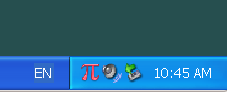
\includegraphics[width=\textwidth]{p-inactive.png}
                      Ἀδρανής
                      % \label{}
                    \end{minipage}
                    \hspace{0.5cm}
                    \begin{minipage}[b]{0.40\linewidth}
                      \centering
                      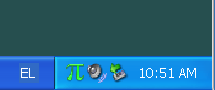
\includegraphics[width=\textwidth]{p-active.png}
                      Ἐνεργός
                      % \label{}
                    \end{minipage}
                    \end{center}
                  \end{figure}

                  \begin{figure}[ht]
                    \begin{center}
                    \begin{minipage}[b]{0.40\linewidth}
                      \centering
                      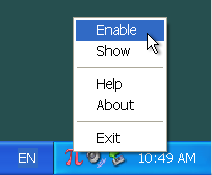
\includegraphics[width=\textwidth]{p-inactive-menu.png}
                      Τὸ μενοῦ ἐλέγχου
                    \end{minipage}
                    \hspace{0.5cm}
                    \begin{minipage}[b]{0.40\linewidth}
                      \centering
                      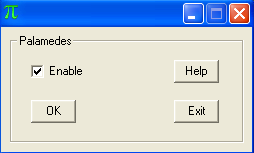
\includegraphics[width=\textwidth]{p-main.png}
                      Ὁ πίναξ ἐλέγχου
                    \end{minipage}

                    \end{center}
                  \end{figure}
    %
    \item{}Πρὶν δακτυλογραφήσουμε ὁτιδήποτε πολυτονικό, βάζουμε τὸ κείμενό 
          μας σὲ μίαν γραμματοσειρὰν Unicode, καὶ γυρίζουμε τὸ πληκτρολόγιον 
          εἰς τὰ Ἑλληνικά.
    %
    \item{}Ὁ Παλαμήδης δεσμεύει τὰ πλῆκτρα \verb|/, \, ~, [, ] | διὰ τὸν
          τονισμόν. Ἐπίσης, ἄλλα εἰδικὰ σύμβολα ὅπως τά ·, ʹ, ͵, 
            Ϝ, Ϟ, Ϡ, €, ϗ, κ.ἄ. εἰσάγονται διὰ τοῦ λεγομένου νεκροῦ πλήκτρου
            «;». Π.χ. διὰ νὰ γράψωμεν «Ϡ» πληκτολογοῦμε ;π (ὅρα πίνακα). Ἂν
            χρειασθοῦμε κάποιο ἐκ τῶν συμβόλων ἅτινα γράφονται διά τῶν δεσμευμένων
            πλήκτρων, τότε προσωρινῶς ἀπενεργοποιοῦμε τὸν Παλαμήδη ἢ γυρίζουμε 
            τὸ πληκτρολόγιον στὰ Ἀγγλικά. 
    %
    \item{}Οἱ τόνοι καὶ τὰ πνεύματα  γράφονται {\bf μετὰ} τὸ γράμμα
            (ὅπως τοὺς γράφουμε μὲ τὸ χέρι) καὶ λειτουργοῦν ἀθροιστικῶς
            δίχως κανόνα προτεραιότητος. Τόνος, πνεῦμα, διαλυτικὰ καὶ
            ὑπογεγραμμένη τίθενται καθ᾽ οἱανδήποτε σειρά. Ἐπὶ παραδείγματι,
            {\large ᾦ} γράφεται μὲ {\large ω]=|} ἢ {\large ω=]|}
            ἢ {\large ω]|=}, κ.λπ. Ὅπου τὸ ] βάζει τὴν Δασεῖα, τὸ
            = βάζει τὴν Περισπωμένη καὶ τὸ | βάζει τὴν Ὑπογεγραμμένη. 
            Ἐπίσης, εἰσαχθέντες τόνοι καὶ πνεύματα  ἐπιδέχονται διορθώσεις·
            ἂν ἐπὶ παραδείγματι θέσαμεν ὀξεῖαν ἀντὶ περισπωμένης, πατώντας
            {\bf$\sim$} ἢ {\bf$=$} ἡ ὀξεῖα θὰ ἀντικατασταθῇ μὲ περισπωμένην.

    %
    \item{}Μεμονωμένοι τόνοι καὶ πνεύματα. (´{ }`{ }῀{ }῭{ }῏, κ.λπ.)  παράγονται
            γράφοντάς τα μετὰ ἀπὸ ἕνα κενὸν διάστημα.
    %
    \item{}Ὁ Παλαμήδης διευκολύνει καὶ τὴν δακτυλογράφηση μονοτονικοῦ
           κειμένου. Ἐν τοιαύτῃ
            περιπτώσει κάνουμε χρῆσιν μόνον τοῦ πλήκτρου τῆς ὀξείας (/).
    %
    \item{}Ὁ Παλαμήδης δύναται νὰ συνυπάρξῃ καὶ εἶναι συμβατὸς μὲ τὸ σύστημα τῶν
            νεκρῶν πλήκτρων τῆς Microsoft.  Π.χ.  τὸ {\bf ά} δύναται νὰ παραχθῇ
            εἴτε μὲ {\bf ;α} εἴτε μὲ {\bf α/}.  Τὸ αὐτὸ ἰσχύει καὶ διὰ τοὺς
            συνδυασμοὺς τοῦ πολυτονικοῦ πληκτρολογίου τῶν Windows
            XP/Vista/7/8.
    %
  \end{itemize}

%%%%%%%%%%%%%%%%%%%%%%%%%%%%%
%     Table
%%%%%%%%%%%%%%%%%%%%%%%%%%%%%
\section*{Πίναξ πληκτρολογίου}
  \newcolumntype{C}{>{\centering\arraybackslash}X}
  \begin{center}
    {\large
      \begin{tabularx}{12cm}{lcC}
      \toprule
      \multicolumn{3}{c}{Τονισμός}                                    \\\midrule
      \multicolumn{2}{c}{Σύμβολον}          & Πλῆκτρον                \\\midrule
      Ὀξεῖα                          & ά    &  \texttt{/}                     \\
      Βαρεῖα                         & ὰ    &  $\backslash$                   \\
      Περισπωμένη                    & ᾶ    &  $\sim$ ἤ =                     \\
      Ψιλή                           & ἀ    &  \texttt{]}                     \\
      Δασεῖα                         & ἁ    &  \texttt{[}             \\\midrule
      \multicolumn{3}{c}{Σημεῖα στίξεως καὶ ἄλλα  σύμβολα}            \\\midrule
      Διαλυτικά                      & ϊ    &  {\tt "}                        \\
      Ὑπογεγραμμένη                  & ᾳ    &  $|$                            \\
      Μακρόν                         & ᾱ    &  $-$                            \\
      Βραχύ                          & ᾰ    &  \textasciicircum               \\ 
      Ἄνω Τελεία                     & ·    &  \texttt{;{\Large .}}           \\
      Τοῖς χιλίοις                   &  ‰   &  \texttt{;\%} \\
      Εὐρῶ                           &  €   &  \texttt{;\$}                   \\
      Ἀριστερὰ Εἰσαγωγικά            &  «   &  \texttt{;{<}}                  \\
      Δεξιὰ Εἰσαγωγικά,              &      &                                 \\
      { }{ }{ }ὁμοιωματικά           &  »   &  \texttt{;{>}}                  \\
      Ἀπόστροφος                     &  ᾽   &  \texttt{;'}                    \\
      Παῦλα τύπου en-dash            &  –   &  \texttt{;-}                    \\
      Παῦλα τύπου em-dash            &  —   &  \texttt{;{\_}}                 \\
      Ἄνω τόνος, κεραία              &  αʹ  &  \texttt{;\#}                   \\
      Κάτω τόνος, χιλιάδες           & ͵α   &  \texttt{;{\small SHIFT}\#}     \\
      Συντομογραφία «καί»            &  ϗ   &  ;κ                             \\
      Στίγμα                         &  Ϛ   &  ;σ                             \\
      Δίγαμμα                        &  Ϝ   &  ;φ                             \\
      Ἀρχαϊκὴ Κόππα                  &  ϙ   &  ;q                             \\
      Βυζαντινὴ Κόππα                &  Ϟ   &  ;Q                             \\
      Σαμπί                          &  Ϡ   &  ;π                  \\\bottomrule
      \end{tabularx}
    }
  \end{center}  
  \vspace{.3cm}
  Σημ. Τὸ «Help» τοῦ μενοῦ ἐμφανίζει αὐτὸν τὸν πίνακα ἐπὶ τῆς ὀθόνης.
\newpage

%%%%%%%%%%%%%%%%%%%%%%%%%%%%%%%%%%%%%%%%%%%%%%%%%%%%%
% Technical info
%%%%%%%%%%%%%%%%%%%%%%%%%%%%%%%%%%%%%%%%%%%%%%%%%%%%%

%%%%%%%%%%%%%%%%%%%%%%%%%%%%%%%%%%%%%%%%%%%%%%%%%%%%%
%  Appendix
%%%%%%%%%%%%%%%%%%%%%%%%%%%%%%%%%%%%%%%%%%%%%%%%%%%%%
\section*{Παλαμήδης ὁ Ναυπλίου}

  Ὁ Παλαμήδης θεωρεῖται ὑπὸ τῶν ἀρχαίων ἐφευρέτης τῶν γραμμάτων, ἔτι δὲ τῶν
  ἀριθμῶν, τῶν μέτρων καὶ σταθμῶν, τῶν νομισμάτων, τῆς διαιρέσεως τοῦ
  χρόνου εἰς ὥρας, ἡμέρας καὶ μῆνας, τῶν στρατιωτικῶν μονάδων ὡς καὶ
  παιγνίων (π.χ. τὸ τάβλι). Ἡ ἀρχαιότερη σωζόμενη μνεία τῆς ἐφευρέσως
  γραμμάτων ἀπὸ τὸν Παλαμήδη εἶναι λατινιστὶ ἀπὸ τὸν Γάιο Ἰούλιο Ὑγῖνο:
  \footnote{Ὑπάρχει ἕνα ἀκόμη, ἀρχαιότερο
      ἀπόσπασμα λόγου τοῦ Γοργία τοῦ Λεοντίνου (Ὑπὲρ Παλαμήδους ἀπολογία) 
      ποὺ ἀναφέρει τὸν Παλαμήδη ὡς ἐφευρέτη τῶν γραμμάτων. Προτιμήσαμε 
      τὸ ἀπόσμασμα τοῦ Ὑγίνου ἐπειδῆ αὐτὸ σκιαγραφεῖ τὴν κατὰ τοὺς ἀρχαίους
      ἱστορία τοῦ Ἀλφαβήτου.}

  \begin{quotation}
    \noindent
    \textit{
          Parcae, Clotho Lachesis Atropos, inuenerunt litteras Graecas
          septem, Α Β Γ Η Τ Ι Υ; alii dicunt Mercurium ex gruum uolatu,
          quae cum uolant litteras exprimunt; Palamedes autem Nauplii
          filius inuenit aeque litteras undecim, Simonides
          litteras aeque quattuor, Ω Ε Ζ Φ, Epicharmus Siculus
          litteras duas, Π et Ψ. has autem Graecas Mercurius in 
          Aegyptum primus detulisse dicitur, ex Aegypto Cadmus in Graeciam, 
          quas Euandrus profugus ex Arcadia in Italiam
        transtulit.}\footnote{Hyginus Gaius Julius (64 π.Χ – 17 μ.Χ.).
          Fabulae. κεφ. 277 (PHI\#5 1263:001) } 
  \end{quotation}    

   Δηλαδή:

  \begin{quotation}
    \noindent
         Οἱ Μοῖρες, Κλωθώ Λάχεσις καὶ Ἄτροπος, ἐπενόησαν τὰ 7 γράμματα,
         Α Β Γ Η Τ Ι Υ· ἄλλοι λέγουν πὼς τὰ ἐφηῦρε ὁ Ἑρμῆς ἀπὸ τὰ σχήματα
         (ποὺ μοιάζουν μὲ τὰ γράμματα) ποὺ κάνουν στὸν οὐρανο ὅταν πετᾶνε 
         οἱ γερανοὶ.
         Παλαμήδης ὁ Ναυπλίου ἐπενόησε 11 γράμματα, ὁ Σιμωνίδης (ὁ Κεῖος)
         ἐπενόησε τὰ Ω Ε Ζ Φ, καὶ ὁ Ἐπίχαρμος ὁ Συρακούσιος τὰ Π καὶ Ψ.
         Λέγεται ὅτι ὁ Ἑρμῆς πῆγε τὰ Ἑλληνικὰ γράμματα στὴν Αἴγυπτο καὶ 
         ἀπὸ ἐκεῖ ὁ Κάδμος τὰ έφερε πάλι στὴν Ἑλλάδα. Εἰς τὴν Ἰταλία 
         τὰ ἔφερε ὁ Εὔανδρος, ὅταν μετανάστευσε ἀπὸ τὴν Ἀρκαδία.
  \end{quotation}    
  \newpage
\section*{Ἐπίλογος}
  Κατὰ τὴν διὰ χειρὸς γραφὴν πρῶτα γράφεται τὸ γράμμα (ἐνίοτε καὶ ὁλόκληρος
  ἡ λέξις) καὶ  ἀκολούθως προστίθενται τὰ σύμβολα τονισμοῦ.  Κατὰ τὴν
  ἠλεκτρονικὴν δακτυλογράφησιν εἴθισται οἱ τόνοι καὶ τὰ πνεύματα νὰ
  εἰσάγωνται πρὶν ἀπὸ τὰ γράμματα, διὰ τῆς μεθόδου τῶν λεγομένων «νεκρῶν
  πλήκτρων» 
  (dead keys),\footnote{
      Τὰ νεκρὰ πλῆκτρα εἶναι κατάλοιπον τῆς ἐποχῆς τῶν μηχανικῶν
      γραφομηχανῶν. Αἱ γραφομηχαναὶ εἶχαν τὸ χαρτὶ στερεωμένο ἐπὶ
      ὁριζοντίου κυλίνδρου ἑλκομένου ὑπὸ μηχανισμοῦ ἐλατηρίου-ἐπισχέστρου
      (καστάνιας) οὕτως ὥστε μὲ κάθε χτύπημα τῶν πλήκτρων ὁ κύλινδρος νὰ
      μετακινῆται αὐτομάτως μίαν θέσιν πρὸς τὰ ἀριστερὰ θέτοντας ὑπό τοῦ
      δρομέος κενὴν θέσιν διὰ τὸ ἑπόμενον γράμμα.  Τὰ τονιζόμενα γράμματα
      ὅμως ἦσαν προβληματικά·  ὁ κύλινδρος  ἔπρεπε νὰ παραμείνῃ ἀκίνητος
      ἵνα τὸ γράμμα στολισθῇ μὲ τὰ διακριτικά του.  Ἡ λύσις ποὺ ἐδόθη ἦταν
      τόνοι καὶ πνεύματα νὰ τυπώνωνται πρὶν ἀπὸ τὸ γράμμα μὲ νεκρὰ πλῆκτρα·
      ἤτοι πλῆκτρα ἀποσυνδεδεμένα ἀπὸ τὸ ἐπίσχεστρον – ἐξ οὗ καὶ τὸ
      «νεκρά».  Ὑπῆρχαν λοιπὸν 3 νεκρὰ πλῆκτρα, ποὺ τύπωναν τόνους καὶ
      πνεύματα ἀφήνοντας τὸν κύλινδρο στὴν ἴδια θέση.  Ἂν καὶ ἀφύσικος,
      αὐτὸς ὁ τρόπος δακτυλογραφήσεως ἧτο  εὔκολος διότι τὰ νέκρα πλῆκτρα
      ἦσαν λίγα καὶ ἐπ’ αὐτῶν ἦταν ἐντυπωμένα τὰ ἀντίστοιχα σύμβολα τονισμοῦ.
      } 
  κατὰ τὸ πρότυπον
  τῶν πάλαι ποτὲ γραφομηχανῶν. Οἱ πρῶτοι ἠλεκτρονικοὶ κειμενογράφοι
  κατεσκευάσθησαν εἰς μίμησιν τῶν γραφομηχανῶν διὰ νὰ μὴν ξενίσουν τοὺς
  τότε δακτυλογράφους καὶ διὰ νὰ διευκολύνουν τὴν ἀποδοχὴν τῶν νέων
  συσκευῶν.

  Σήμερον οὐδεὶς λόγος συντρέχει οἱ ἠλεκτρονικοὶ ὑπολογιστῆρες\footnote{
    Ὑπολογιστὴρ εἶναι ὁ ὑπολογίζων μηχανισμός, ὑπολογιστὴς εἶναι
    ὁ ὑπολογίζων (τὸ συμφέρον του) ἄνθρωπος, ὁ συμφεροντολόγος· βλέπε τὰ
    ὑαλοκαθαριστήρ - ὑαλοκαθαριστής, κινητήρ, ὁδοστρωτήρ, ἀνεμιστήρ,
    ἀναπτήρ, κ.λπ. Δὲν γράφουμε κινητής, ὁδοστρωτής, ἀνεμιστής, ἀναπτής.
  } νὰ ἐξακολουθοῦν νὰ μιμοῦνται τὰς γραφομηχανάς, ὅταν αἱ γραφομηχαναὶ
  ἔχουν καταργηθῇ πρὸ εἰκοσαετίας καὶ πλέον.  Ἀκόμη καὶ διὰ μονοτονικὰ
  κείμενα ἡ μέθοδος τῶν νεκρῶν πλήκτρων εἶναι δυσχερής.  Ἕνα μειονέκτημα
  τῆς μεθόδου αὐτῆς εἶναι ἡ δυσκολία κατὰ τὴν διόρθωσιν.  Ἂν ἐν τῇ ρύμῃ τῆς
  γραφῆς παραλειφθῇ ἕνας τόνος, ἡ διόρθωσις ἀπαιτεῖ σβήσιμο τοῦ γράμματος
  καὶ ἐκ νέου εἰσαγωγὴ τοῦ συνδυασμοῦ τόνος-γράμμα.  Τὰ δὲ πληκτρολόγια δὲν
  ἔχουν τυπωμένα στὰ πλῆκτρα τὰ σύμβολα τονισμοῦ. Ὁ χειριστὴς πρέπει νὰ
  θυμᾶται ὅτι ὁ τόνος εἰσάγεται μὲ τὸ πλῆκτρον {\bf;}  καθὼς ἐπίσης τὰ
  πλῆκτρα γιὰ τὰ διαλυτικά, τὸ Ἑλληνικὸν ἐρωτηματικόν, τὴν ἄνω καὶ κάτω
  τελεία κλπ. Πόσοι ἄραγε θυμοῦνται τὸν συνδυασμὸν πλήκτρων γιὰ τὰ
  διαλυτικὰ μὲ τόνο; Πολλῷ μᾶλλον, ξέρει κανεὶς πῶς εἰσάγεται ἡ ἄνω τελεία;

  Ἡ πολυτονικὴ δακτυλογράφησις, ὅταν εἶναι δυνατή, εἶναι ἔτι δυσκολωτέρα καὶ
  ἀπαιτεῖ ἀπομνημόνευσιν 20 - 25 (!) διαφορετικῶν συνδυασμῶν νεκρῶν
  πλήκτρων.\footnote{Διὰ τοῦ λόγου τὸ ἀληθὲς διαβάστε τὶς ὁδηγίες τῆς Microsoft 
  γιὰ τὸ πολυτονικὸ πληκτρολόγιο:\\
  \texttt{http://www.jcu.edu/language/llc/keyboard-setup-greek.htm}\\
  \texttt{\scriptsize{http://download.microsoft.com/download/2/5/4/2543a817-a8c4-4c63-a46a-f04a82bf623e/The Greek Polytonic System.doc}}} 
  Τὰ παραγόμενα σύμβολα δὲν ἔχουν λογικὴν ἀντιστοιχίαν μὲ τὰ λατινικὰ σύμβολα τῶν
  πλήκτρων καὶ ὁ χειριστὴς χρειάζεται νὰ ἔχῃ πρόχειρον πίνακα
  ἀντιστοιχίας πλήκτρων-συμβόλων.

  Μεθ’ ὅλα ταῦτα, ἡ δακτυλογράφησις τῶν Ἑλληνικῶν γίνεται στρυφνή,
  χρονοβόρος καὶ ἐπίπονος. Αἱ δυσκολίαι αὐταὶ παρέχουν δικαιολογίας καὶ
  προφάσεις εἰς ὅσους πρεσβεύουν ὅτι ὁ γραπτὸς λόγος πρέπει νὰ ἀπλοποιῆται
  τάχα πρὸς χάριν τῶν ὑπολογιστήρων.  Ὡς ἀποτέλεσμα βλέπουμε τὴν λυπηρὰν
  διολίσθησιν ἀπὸ τὸ πολυτονικὸν εἰς τὸ μονοτονικόν, κατόπιν εἰς τὸ
  ἀτονικὸν καὶ τέλος εἰς τὴν φρίκην τῆς λατινογράμματης Ἑλληνικῆς.

  Ἴσως ἡ ἁπλούστευσις νὰ ἦτο ἀναγκαία τὴν ἐποχὴν τῶν πρώτων ὑπολογιστήρων,
  οἵτινες ἦσαν ἐπιστημονικαὶ ἢ λογιστικαὶ συσκευαὶ περιορισμένων
  δυνατοτήτων.  Οἱ ἐξελιγμένοι ὑπολογιστῆρες τῆς σήμερον ὅμως ἔχουν
  πλεῖστες δυνατότητες.  Μποροῦν νὰ ἐπεξεργάζωνται ἦχον καὶ εἰκόνα καὶ νὰ
  γράφουν περίπλοκες γραφὲς ὅπως τὰ Κινεζικὰ καὶ τὰ Ἀραβικά. Ἡ εἰσαγωγὴ
  Ἑλληνικοῦ κειμένου κατὰ τὸν τρόπον τῆς διὰ χειρὸς γραφῆς εἶναι ἐν
  συγκρίσει ἁπλουστάτη (καθὼς καταδεικνύεται διὰ τοῦ Παλαμήδους).  Οἱ
  ὑπολογιστῆρες μποροῦν πλέον καὶ πρέπει νὰ εἶναι ἀρωγοὶ εἰς τὰς ἐργασίας
  μας, ἄνευ τῆς ἀνάγκης νὰ υἱοθετοῦμε πρὸς χάριν των δυσχερεῖς τε καὶ
  ἀφύσικους τρόπους γραφῆς.

  Ὁ Παλαμήδης εἶναι μία προσπάθεια πρὸς τὴν ἐξεύρεσιν τρόπου διὰ τὴν εὔκολον 
  δακτυλογράφησιν τῆς παραδοσιακῆς γραφῆς, οἵαν προτιμοῦμε ὡς πλέον
  καλαίσθητη. Ἂν καὶ οὐδ᾽ ὅλως τὸ σκοπεύαμε, παράπλευρον ὄφελος τῆς προσπαθείας 
  ταύτης εἶναι καὶ ἡ εὐκολωτέρα μονοτονικὴ γραφή.

  Ἐλπίζομεν εἰς τὸ μέλλον νὰ ὑπάρξουν καὶ ἄλλα προγράμματα\footnote{Ὑπάρχει
  πρόγραμμα ἀντίστοιχον τοῦ Παλαμήδους διὰ τὸν κειμενογράφον (editor) vim/gvim
  καὶ διατίθεται ἐπίσης δωρεάν.
  http://www.vim.org/scripts/script.php?script\_id=2743} διὰ τὴν σωστὴν
  γραφὴν τῆς῾Ελληνικῆς, καθὼς καὶ πολυτονικοὶ διορθωταὶ
  κειμένου,\footnote{Ὁ Vim ἐπίσης ἔχει καὶ πολυτονικὸν ὁρθογραφηστῆρα.\\
  Βλέπε: http://www.vim.org/scripts/script.php?script\_id=3388} εὑρετήρια
  ρηματικῶν τύπων,\footnote{http://www.kalos-software.com} κ.ἄ.

\end{document}
